\documentclass{beamer}

\usepackage{amsmath}
\usepackage[style=alphabetic,url=true]{biblatex}
\usepackage{environ}
\usepackage{geometry}
\usepackage{graphicx}
\usepackage{listings}
\usepackage{tikz}
\usepackage{tkz-graph}
\usepackage[T2A]{fontenc}
\usepackage[utf8]{inputenc}
\usepackage[scaled=0.9]{DejaVuSansMono}

\pagenumbering{arabic}
\graphicspath{ {./graphics/} }
\setbeamertemplate{itemize item}[circle]
\setbeamertemplate{itemize subitem}{--}
\addtobeamertemplate{navigation symbols}{}{
  \usebeamerfont{footline}%
  \usebeamercolor[fg]{footline}%
  \hspace{1em}%
  \insertframenumber/\inserttotalframenumber
}
% \usetheme{Bergen}
% \usecolortheme{beaver}

\lstset{frame=tb,
  language=Lisp,
  basicstyle=\scriptsize\ttfamily,
  keywordstyle=\color{teal},
  commentstyle=\color{gray},
  frame=none,
  % aboveskip=3mm,
  % belowskip=3mm,
  % showstringspaces=false,
  % columns=flexible,
  % numbers=none,
  % stringstyle=\color{mauve},
  % breaklines=true,
  % breakatwhitespace=true,
  % tabsize=3
}

\title{CLOS \& MOP}
\subtitle{Common Lisp Object System \& Metaobject Protocol}
\author{ Жикін Юрій \\ \url{whythat@protonmail.com}}
\date{18 травня, 2020}


\begin{document}

\frame{\titlepage}

\begin{frame}[fragile]
  \frametitle{CLOS: Common Lisp Object System}
  \begin{itemize}
  \item При підготовці стандарту ANSI Common Lisp у 1980-х запропонована як
    альтернатива більш раннім об'єктним системам \textit{MIT Flavors} та
    \textit{CommonLoops} в старіших мовах сімейства Lisp.
  \item Вся об'єктна система складається з трьох основних макросів
    (\texttt{defclass}, \texttt{defgeneric} та \texttt{defmethod}) та декількох
    функцій.
  \end{itemize}
\end{frame}

\begin{frame}[fragile]
  \frametitle{CLOS: термінологія}
  \begin{itemize}
  \item \textbf{Загальна функція} (англ. \textit{generic function}) - функція,
    реалізація якої обирається динамічно залежно від типів її параметрів (так
    званий \textit{динамічний поліморфізм}).
  \item \textbf{Метод} (англ. \textit{method}) - конкретна реалізація
    \textit{загальної функції} для певної комбінації типів її параметрів.
  \item \textbf{Діючий метод} (англ. \textit{effective method}) - метод, обраний
    під час виконання програми залежно від фактичних аргументів
    \textit{загальної функції}.
  \item \textit{Загальну функцію} можна розглядати як множину методів та правило
    вибору \textit{діючого методу}.
  \end{itemize}
\end{frame}

\begin{frame}[fragile]
  \frametitle{CLOS: класи та об'єкти}
  \begin{itemize}
  \item Класи оголошуются за допомогою форми \texttt{defclass}:
    \begin{lstlisting}
  (defclass shape () ())

  (defclass square (shape)
    ((side :accessor square-side 
           :initarg :side)))

  (defclass circle (shape)
    ((radius :accessor circle-radius 
             :initarg :radius)))
    \end{lstlisting}
  \item Створити об'єкт класу можна за допомогою функції \texttt{make-instance}:
    \begin{lstlisting}
  (make-instance 'circle :radius 4)
    \end{lstlisting}
  \end{itemize}
\end{frame}

\begin{frame}[fragile]
  \frametitle{CLOS: загальні функції та методи}
  \begin{itemize}
  \item Загальні функції оголошуються за допомогою форми \texttt{defgeneric}:
    \begin{lstlisting}
  (defgeneric perimeter (shape))
    \end{lstlisting}
  \item Методи загальних функцій додаються формою \texttt{defmethod}:
    \begin{lstlisting}
  (defmethod perimeter ((shape square))
    (* 4 (square-side shape)))

  (defmethod perimeter ((shape circle))
    (* 2 pi (circle-radius shape)))
    \end{lstlisting}
  \item Аналогічний приклад у мові Python:
    \begin{lstlisting}[language=Python]
  class Square:
      def perimeter(self): 
          return 4*self.side
    \end{lstlisting}
  \end{itemize}
\end{frame}

\begin{frame}[fragile]
  \frametitle{CLOS: інтерфейси та мультиметоди}
  \begin{itemize}
  \item Методи \textbf{не} є компонентами класів, тому інтерфейси в CLOS
    оголошуються як набір загальних функцій:
    \begin{lstlisting}
  ;; Graph interface.
  (defgeneric node-payload (graph node))
  (defgeneric previous-nodes (graph node))
  (defgeneric next-nodes (graph node))
    \end{lstlisting}
  \item Методи в CLOS можуть бути спеціалізовані відносно кількох параметрів --
    такий тип методів називають \textbf{мультиметодами}:
    \begin{lstlisting}
  (defgeneric link-nodes (n1 n2))

  (defmethod link-nodes ((n1 simple-node) (n2 simple-node))
    (add--line n1 n2))

  (defmethod link-nodes ((n1 simple-node) (n2 comment-node))
    (add-dashed-line n1 n2))
    \end{lstlisting}
  \end{itemize}
\end{frame}

\begin{frame}[fragile]
  \frametitle{CLOS: допоміжні методи}
  \begin{itemize}
  \item CLOS дозволяє оголошувати методи, що адаптують існуючі методи,
    виконуючись перед, після чи ``навколо'' основного метода (модифікатори
    \texttt{:before}, \texttt{:after} та \texttt{:around}, відповідно):
    \begin{lstlisting}
  (defmethod make-instance ((class class) &rest args)
     ...)

  ;; First find the class object and then call 
  ;; the method above with it.
  (defmethod make-instance :around ((name symbol) &rest args)
    (funcall #'call-next-method (find-class c) args))
    \end{lstlisting}
  \end{itemize}
\end{frame}

\begin{frame}[fragile]
  \frametitle{MOP: Metaobject Protocol}
  \begin{itemize}
  \item Система CLOS стала відома поза спільнотою користувачів Common Lisp
    завдяки книзі ``Мистецтво метаоб'єктного протоколу'' (Г. Кічалес, Дж. де
    Рів'єр та Д. Бобров), яку ідеолог об'єктно-орієнтованого програмування Алан
    Кей назвав ``найкращою книгою за останні 10 років''.
  \end{itemize}
  \begin{center}
    \includegraphics[scale=0.2]{amop}
  \end{center}
\end{frame}

\begin{frame}[fragile]
  \frametitle{MOP: для чого?}
  \begin{itemize}
  \item Принцип відкритості/закритості Бертрана Мейєра:
    \par\textit{``об'єктні системи повинні бути відкритими для розширення, але
      закритими для модифікації''.}
  \item Один з основних принципів дизайну мови Common Lisp:
    \par\textit{``користувач мови повинен мати змогу робити все, що може робити
      розробник мови''.}
  \item MOP задовільняє обидва принципи, подаючи саму об'єктну систему CLOS як
    набір CLOS-об'єктів.
  \item MOP доповнює макро-систему Common Lisp:
    \begin{itemize}
    \item макро-система дозволяють користувачу створювати нові синтаксичні
      конструкції;
    \item метаоб'єктний протокол дозволяє користувачу створювати нові об'єктні
      системи.
    \end{itemize}
  \end{itemize}
\end{frame}

\begin{frame}[fragile]
  \frametitle{MOP: простір об'єктних систем}
  \begin{itemize}
  \item MOP можна розглядати як область у просторі об'єктних систем, де самі
    об'єктні системи розглядаються як точки:
  \end{itemize}
  \begin{center}
    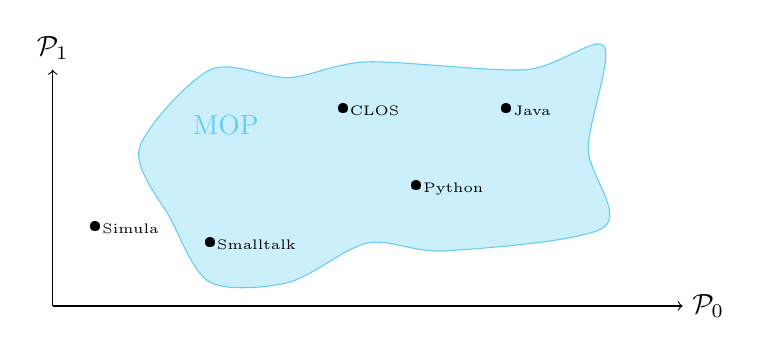
\begin{tikzpicture}
      \draw [->] (0, 0) -- (0, 3) node[above] {$\mathcal{P_\text{1}}$};
      \draw [->] (0, 0) -- (8, 0) node[right] {$\mathcal{P_\text{0}}$};
      \draw [cyan!60, fill=cyan!20] plot [smooth cycle] coordinates {
        (1.5, 1.1) (1.1, 2) (2, 3) (3, 2.9) (4, 3.1) (6, 3) (7, 3.3)
        (6.8, 2) (7, 1) (5, 0.7) (4, 0.8) (3, 0.3) (2, 0.3)
      } node at (2.2, 2.3) {MOP};
      \node at (0.9, 1)     {\textbullet \tiny{Simula}};
      \node at (2.5, 0.8) {\textbullet \tiny{Smalltalk}};
      \node at (4, 2.5)   {\textbullet \tiny{CLOS}};
      \node at (5, 1.5)   {\textbullet \tiny{Python}};
      \node at (6, 2.5)   {\textbullet \tiny{Java}};
    \end{tikzpicture}
  \end{center}
\end{frame}

\begin{frame}[fragile]
  \frametitle{MOP: як це працює?}
  \begin{itemize}
  \item Оголошення класів та загальних функцій зберігаються у глобальних
    реєстрах у вигляді об'єктів \texttt{class} та \texttt{generic-function}
    відповідно.
  \item Оголошення методів зберігаються у вигляді об'єктів типу \texttt{method}
    об'єктах \texttt{generic-functions}.
  \item Кожен новий клас додається у списки предків/нащадків відповідних
    класів. Ці списки фіксуються у якийсь момент перед створенням першого
    екземпляру класу.
  \item На основі списків пріоритету предків та списків методів для кожної
    загальної функції \textit{будується} \textbf{функція-дискримінант}, яка
    реалізує вибір діючого методу залежно від аргументів.
  \item Під час виклику загальної функції викликається
    \textit{функція-дискримінант}, яка обирає та викликає відповідний діючий
    метод.
  \end{itemize}
\end{frame}

\begin{frame}[fragile]
  \frametitle{MOP: об'єктно-орієнтований протокол}
  \begin{itemize}
  \item В більшості реалізацій Common Lisp всі компоненти CLOS реалізовані як
    набір класів (метакласів), загальних функцій та методів CLOS.
  \item Спадкуючи нові метакласи від стандартних MOP-класів та перевантажуючи
    методи MOP, можна створювати нові об'єктні системи, що краще підходять для
    відповідної предметної області.
  \item Практичний приклад - оптимізація об'єктної системи.
  \item Приклад з історії - деякі legacy-бази коду, що використовували старіші
    мови Lisp занадто сильно залежали від деталей реалізації об'єктної системи
    Flavors, тому розробники портували їх на Common Lisp з адаптованою за
    допомогою MOP об'єктною системою, що поводилась як Flavors.
  \end{itemize}
\end{frame}

\begin{frame}[fragile]
  \frametitle{CLOS\&MOP: на завершення}
  \begin{itemize}
  \item CLOS - надзвичайно гнучка об'єктна система, що надає користувачу більше
    свободи та можливостей ніж більшість існуючих об'єктних систем в
    мейнстрімових мовах програмування.
  \item MOP розділяє функціональну та процедурну складові об'єктоно орієнтованої
    системи, відкриваючи можливості для оптимізацій, що не потребують змін в
    роботі компілятора.
  \item Окрім того, MOP має академічне застосування як платформа для
    експериментів з властивостями об'єктних систем.
  \end{itemize}
\end{frame}

\begin{frame}[fragile]
  \begin{center}
    \huge{Дякую за увагу!}
  \end{center}
\end{frame}

\printbibliography
\end{document}
